\documentclass{article}
\usepackage{amsmath,graphicx,amsfonts,amssymb,amsthm,hyperref,amscd}
\setcounter{MaxMatrixCols}{30}
\usepackage{tikz-cd}
\setcounter{tocdepth}{10}
\providecommand{\U}[1]{\protect\rule{.1in}{.1in}}
\setlength{\topmargin}{-1.0in}
\setlength{\textheight}{9.25in}
\setlength{\oddsidemargin}{0.0in}
\usepackage{mathtools}
\setlength{\evensidemargin}{0.0in}
\setlength{\textwidth}{6.5in}
\def\labelenumi{\arabic{enumi}.}
\def\theenumi{\arabic{enumi}}
\def\labelenumii{(\alph{enumii})}
\def\theenumii{\alph{enumii}}
\def\p@enumii{\theenumi.}
\def\labelenumiii{\arabic{enumiii}.}
\def\theenumiii{\arabic{enumiii}}
\def\p@enumiii{(\theenumi)(\theenumii)}
\def\labelenumiv{\arabic{enumiv}.}
\def\theenumiv{\arabic{enumiv}}
\def\p@enumiv{\p@enumiii.\theenumiii}
\pagestyle{plain}
\parindent=0pt
\newcommand{\Z}{\mathbb{Z}}
\newcommand{\B}{\beta}
\newcommand{\A}{\alpha}
\newcommand{\N}{\mathbb{N}}
\newcommand{\Ha}{\mathbb{H}}
\newcommand{\C}{\mathbb{C}}
\newcommand{\R}{\mathbb{R}}
\newcommand{\F}{\mathbb{F}}
\newcommand{\Q}{\mathbb{Q}}
\newcommand{\Oa}{\mathcal{O}}
\newcommand{\K}{\mathcal{K}}
\newcommand{\as}{\text{*}}
\newcommand{\tr}{\text{tr}}
\newcommand{\dt}{\bullet}

\newtheorem{theorem}{Theorem}[subsection]
\newtheorem{exercise}[theorem]{Exercise}
\newtheorem{example}[theorem]{Example}
\newtheorem{corollary}[theorem]{Corollary}
\newtheorem{lemma}[theorem]{Lemma}
\newtheorem{proposition}[theorem]{Proposition}
\theoremstyle{definition}
\newtheorem{definition}[theorem]{Definition}
\newtheorem{remark}[theorem]{Remark}
\newtheorem*{claim}{Claim}
\newtheorem{axiom}{Axiom}

\usepackage[english]{babel}
\usepackage[utf8]{inputenc}

\usepackage{caption}
\usepackage{subcaption}
\usepackage{wrapfig}

\title{Felipe Gutierrez}
\date{}
\author{Statement of Purpose}
\begin{document}
\maketitle 

I am an undergraduate student in the AMEP (Applied Math, Engineering and Physics) and Computer Science (CS) programs at the University of Wisconsin-Madison. During my time at UW-Madison, I explored topics in computer science, math, physics and engineering. I developed a degree of maturity in research, experienced industry through an internship, and collaborated in software and research projects with professors and graduate students. Motivated to build on this background, I would like to be considered for the EECS Ph.D. training program at the Massachusetts Institute of Technology.

\section*{Undergraduate Academic Experience}

\subsection*{Coursework}
UW-Madison has given me the opportunity to explore basic to advanced courses in computer science, math, physics, mechanical and electrical engineering. For example, Stochastic Processes (Math605), gave me the tools to approach real life modeling problems using probability theory. Computational Dynamics of Machine Systems (ME451) gave me the opportunity to write my first 10,000+ line program, a simulation engine for kinematic and dynamic analysis. Furthermore, I went through the traditional computer science curriculum. This included theory courses such as Algorithms and Discrete Math (CS577, CS240), that exposed me to the foundational blocks that link computer science to mathematics, and it also included applied courses like Databases (CS564), where I learned how to design an application around the available data to make implementation and support run smoothly. Finally, to complete the honors option in computer science, I took graduate courses including Computational Cognitive Sciences (CS841), where I built a lightness illusion detector. Hence, the broad spectrum of courses I took during my undergraduate career exposed me to different research areas. \newline

My undergraduate training covered a breadth of topics in applied sciences. This being said, I was also able to acquire depth in a number of topics through the research projects that I was involved in. In the next sections, I will describe these projects.

\begin{wrapfigure}{r}{0.5\textwidth}
    \vspace{-23pt}

  \begin{center}
    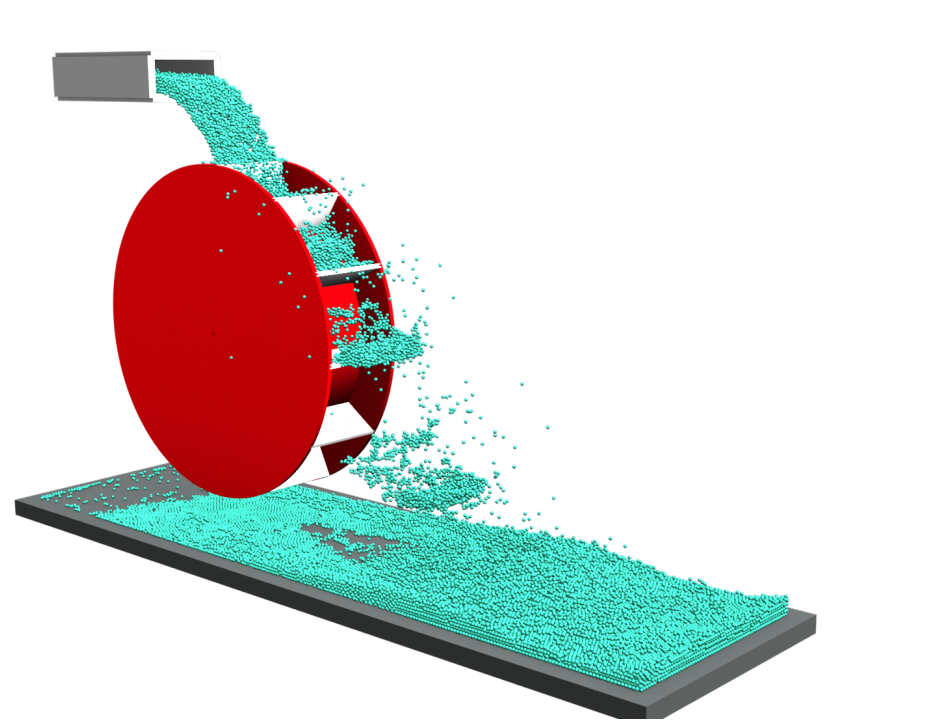
\includegraphics[width=0.48\textwidth, height=5cm]{waterwheel.png}
  \end{center}
   \vspace{-15pt}

  \caption{Waterwheel simulation rendered with Chrono::Render.}\label{Fig:foam}
   \vspace{-5pt}

\end{wrapfigure}

\subsection*{Web Interface for Chrono::Render}
During my sophomore year, I collaborated with Professor Dan Negrut on a project called Chrono::Render. We developed a graphical visualization pipeline for generating high quality videos and images from multibody dynamics simulations, such as the one in Figure \ref{Fig:foam} \cite{chronoRender}. Moreover, the tool gives users the option to quickly render each frame of their simulation in parallel using the lab's cluster \cite{eulerCluster}. We used Blender \cite{blender1, blender2} as the front-end to generate config files which Chrono::Render processes and sends to a rendering toolkit, such as Pixar's PRMan \cite{prman}. I developed the web interface that was used to submit the rendering jobs to the cluster. Our work was presented at IDETC/CIE 2014 \cite{chronoRender}. 

\newpage



\subsection*{Modeling and Simulation of Fluid-Solid Interaction (FSI) problems}


\begin{wrapfigure}{r}{0.5\textwidth}
    \vspace{-23pt}

  \begin{center}
    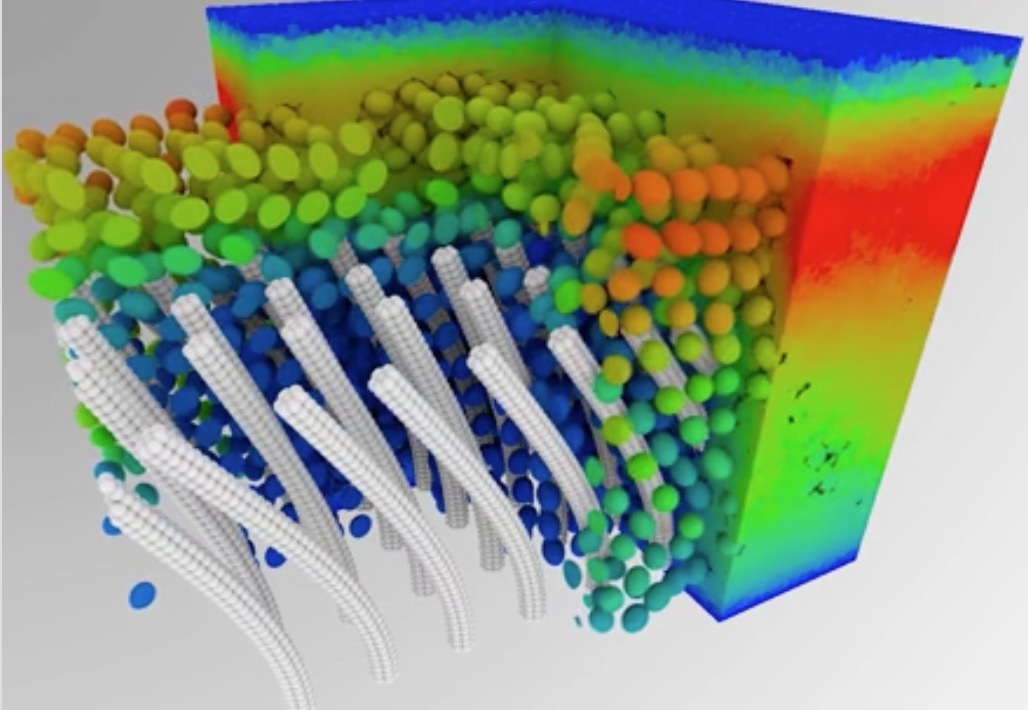
\includegraphics[width=0.48\textwidth, height=5cm]{fsi.png}
  \end{center}
    \vspace{-15pt}

  \caption{Chrono::FSI simulation of flexible beams and rigid ellipsoids in a fluid.}\label{Fig:fsi}
  \vspace{-10pt}
\end{wrapfigure}


My junior year, I was accepted into the Blue Waters Student Internship Program (BWSIP) \cite{bwsip}. The BWSIP is an initiative from the National Center for Supercomputing Applications (NCSA) to advance scientific computing through High-Performance Computing (HPC). As a pre-requisite for my internship, I attended a two-week HPC workshop at the University of Illinois Urbana-Champaign. For my research project, I collaborated with Dr. Arman Pazouki and Professor Negrut in a study of parallel computing tools/techniques and their implementation to FSI problems. Specifically, we developed a simple Computational Fluid Dynamics (CFD) MATLAB code based on Smoothed Particle Hydrodynamics (SPH). This is used as a prototyping environment for boundary conditions and numerical methods. Next, I became a core developer of the CUDA-based SPH code in Chrono::FSI \cite{chronoFSI}, a module of Chrono which is an open source multi-physics engine \cite{chrono}. Chrono::FSI has been used to create simulations such as the one in Figure \ref{Fig:fsi}. Most recently, we have been working on developing a distributed memory FSI engine using the Charm++ parallel programming framework. This framework uses multiple nodes; thus we can fully capture the interaction of the fluid and solid in large and multi-scale FSI problems. One such problem is modeling articular cartilage where millions of flexible bodies interact in tissue fluid. I will be presenting this work in IDETC/CIE 2016.



\subsection*{Permutation Testing in Neuroimaging Datasets}

At the end of my junior year, after completing my final project for Computer Vision (CS766), I started collaborating as a research assistant with Professor Vikas Singh on topics related to statistical analysis of brain imaging datasets. In neuroimaging studies, voxel-by-voxel hypothesis testing is often used  to locate statistically significant brain regions that display high activity and/or group differences \cite{Holmes96}. Permutation testing is a nonparametric computationally expensive algorithm that is used to locate these regions \cite{Holmes96, Nichols02, Ithapu13}. My work was based on the simple idea provided in \cite{Ithapu13}, which exploited the problem structure to reduce computation time in permutation testing. The procedure in \cite{Ithapu13} was only tested in small datasets and mainly served as a proof-of-concept. Building upon this algorithm, my work has been three-fold. The first step was to improve the scalability of the algorithm to large datasets while still maintaining strong computational gains. Secondly, the procedure was to be extensively compared to the widely used multiple hypothesis testing toolbox, SnPM\cite{SnPM}, and augment it with snippets of the algorithm. Lastly, the algorithm was extended to support a wide-variety of hypothesis testing regimes (one-sample, two-sample etc.). To address these goals, I reformulated the algorithm by exploiting certain matrix factorization aspects of the permutation testing procedure, including a parallelizable step that was ignored in its earlier version. Overall, the new implementation displayed promising performance, both in terms of applicability to large datasets and comparisons to SnPM. Summarizing these observations, I am currently leading an effort to prepare a detailed manuscript for submission to a high-impact journal. I intend to complete the submission and release an open-source version of the extended algorithm in the coming few weeks. I plan to further involve myself in other research projects in Professor Singh's group. 

\subsection*{Teaching Experience}

Throughout my senior year, I have assisted Professor Negrut in a high performance computing course (ECE759) \cite{me759}. I had the opportunity to prepare various materials which he has utilized for the course. In addition, I helped two graduate students plan their final projects and solve technical issues that they came across. I have also been mentoring an undergraduate student in SPH-based CFD. I have experienced that teaching helps me internalize the concepts that I have previously learned, making it an enjoyable and rewarding experience.

\section*{Looking Ahead - Graduate School Aspirations}

In conclusion, I want to dedicate the next years of my career to pursue a Ph.D. in the EECS department at MIT. I am particularly interested in the EECS program because I believe it will provide me with strong theoretical foundations for my research in applied problems. I want to further my studies in scientific computing, physics-based modeling and simulation, and machine and statistical learning to eventually become a multi-disciplinary researcher. One of my interests lies at the intersection of scientific computing and physics-based modeling; I am interested in research problems that come up when trying to efficiently and accurately model multi-scale, multiphysics systems; specifically in biophysical systems. Furthermore, I have a keen interest in how these models can be jointly used with patient specific medical data to produce accurate diagnostics and to plan medical procedures. In a similar context, I am interested in learning how to use mathematical and statistical tools to extract as much information as possible from medical data and train models that can aid diagnostics. With these interests in mind, I am excited to have found the Biomedical Science and Engineering focus area in EECS which make the program completely align with my goals and research interests. If given the opportunity to join the MIT community I believe that I will be able to expand my knowledge and make impactful contributions in the above research areas.\linebreak

I want to thank the selection committee for your consideration in the review of this application.\linebreak
\linebreak
Respectfully,\linebreak
Felipe Gutierrez


\bibliographystyle{unsrt}
\bibliography{felipe_sop_bib}


\end{document}




